\documentclass[a4paper, 11pt]{article}

\usepackage{caption}
\usepackage{enumitem}
\usepackage{graphicx}
\usepackage{hyperref}
\usepackage[utf8]{inputenc}
\usepackage{minted}

\begin{document}

\title{
	\textbf{Hash Tables in C}
}
\author{Neo Gullberg}
\date{Fall 2024}
\maketitle

\section{Introduction}
	For this assignment my task was to implement functionality for working with hash tables in the C programming language.
	If implemented correctly, hash tables can contribute to blazingly fast access times for stored data.
	Hash tables work similarly to arrays, in that you only need to specify a key (similar to an index in an array) to near instantly retrieve the value you want.
	It is therefore a very useful tool for any programmer to add to their toolbox.

\section{Swedish Zip Codes}
	We were given a data set of swedish zip codes in a CSV (comma separated value) file, each with a corresponding area name and population.
	These were to be used to test out our hash table implementations.
	In total there were 9675 zip codes, all in the range of [111 15, 984 99].
	A naive approach to storing this data would be to create an array of size 98500 (so that the last index corresponds to 98499)
	and have each entry get an index in the array corresponding to their own zip code.
	This would indeed give us blazingly fast access speeds, with the downside of almost 90\% of the array being left unused.
	But it will still be good to benchmark this so that we have something to compare against further down the road.
	\par
	To start, we were asked to benchmark three different ways to access the zip codes: \textit{Linear search}, \textit{Binary search}, and \textit{Array accesses}.
	For each one we were also to compare the differences between representing the zip codes as strings (\texttt{char *}) as opposed to integers (\texttt{int}).

	\begin{minipage}{0.45\textwidth}
		\centering
		\captionof{table}{\texttt{char *} datatype}
		\begin{tabular}{|c|c|c|}
			\hline
			\textbf{Zip Code} & \textbf{111 15} & \textbf{984 99} \\
			\hline
			Linear & 4.1 & 25268.1 \\
			\hline
			Binary & 443.4 & 397.1 \\
			\hline
			Access & 18.0 & 17.1 \\
			\hline
		\end{tabular}
	\end{minipage}
	\begin{minipage}{0.45\textwidth}
		\centering
		\captionof{table}{\texttt{int} datatype}
		\begin{tabular}{|c|c|c|}
			\hline
			\textbf{Zip Code} & \textbf{111 15} & \textbf{984 99} \\
			\hline
			Linear & 1.5 & 4730.7 \\
			\hline
			Binary & 20.6 & 19.3 \\
			\hline
			Access & 0.2 & 0.2 \\
			\hline
		\end{tabular}
	\end{minipage}

	We see that, for all cases, the integer representation is always faster.
	This is to be expected since integer comparisons are much faster than for strings.
	However, there are also many similarities between the two.
	For linear search the time it takes to find 111 15 is almost instant, while it takes substantially longer to find 984 99.
	This is to because 111 15 is the first element in the array, whilst 984 99 is the last.
	This means they are equally far apart from the middle, which is why binary search takes almost exactly the same amount of time.
	When it comes to array accesses, which mimics the behaviour of a hash map, the times are basically the same, and near instant.

\section{Hash Functions}
	In the last section we saw the benefits of accessing via an array, but the problem we ran into was that it resulted in a bunch of wasted space.
	We have around 10 000 values to map out, and we want to try and find the best way to limit the zip codes to a certain range whilst also minimizing the space needed.
	What we are searching for is a so called hash function.
	That is, a function that takes in a key and spits out an index.
	A simple hash function can be made by taking a value modulo some other value \textit{m}.
	However, the problem with this is that certain keys may transform into the same index, which results in a so called \textit{collision}.
	I made a function to calculate the number of collisions for a given modulo value and also made a graph of the results:
	\begin{figure}[H]
		\centering
		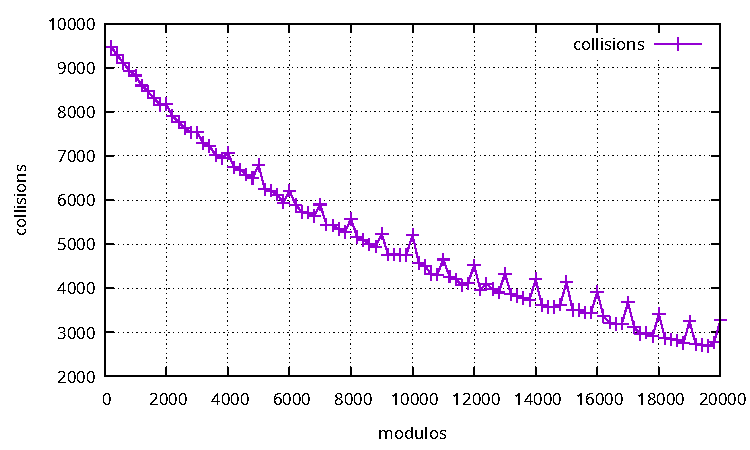
\includegraphics[scale=0.8]{graphs/collisions.pdf}
		\caption{
			Graph showing the number of collisions for various modulo values.
		}
	\end{figure}
	There are a few spikes here and there, but over a longer period it seems to follow a general downwards trend.
	There were also a couple of specific values we were asked to examine:

	\begin{center}
		\captionof{table}{Specific modulo values and their corresponding number of collisions.}
		\begin{tabular}{|c|c|}
			\hline
			\textbf{Modulo} & \textbf{Collisions} \\
			\hline
			10000 & 5210 \\
			\hline
			20000 & 3271 \\
			\hline
			12345 & 2529 \\
			\hline
			17389 & 1745 \\
			\hline
			13513 & 2288 \\
			\hline
			13600 & 3780 \\
			\hline
			14000 & 4203 \\
			\hline
		\end{tabular}
	\end{center}
	\par
	Like we saw in the graph, a bigger modulo value does not always equal less collisions.
	The values 10 000 and 20 000 look to be the tip of spikes as seen in the graph.
	Out of all the measurements in the graph I got that mod 19412 had the fewest number of collisions at 1242.

\section{Buckets}
	Of course we want to avoid confusing two different keys with the same value.
	This can be solved in multiple ways, on of the easiest being with a so called bucket approach which we will start of with.
	A bucket contains different values that all map to the same key.
	In our case it is represented as an array.
	This does not remove collisions completely, but it ensures we can distinguish between different elements.
	If we now want to check whether or not our hash map contains a certain value we follow this process:
	\begin{enumerate}
		\item Convert our value to an index via our hash function.
		\item Go to the corresponding bucket.
		\item Loop through all elements in the bucket and check whether or not the bucket contains what we are looking for.
	\end{enumerate}
	If the number of buckets is large enough we should expect the number of loop throughs to decrease.
	To test this I graphed the average loop throughs for a varying number of buckets.
	\begin{figure}[H]
		\centering
		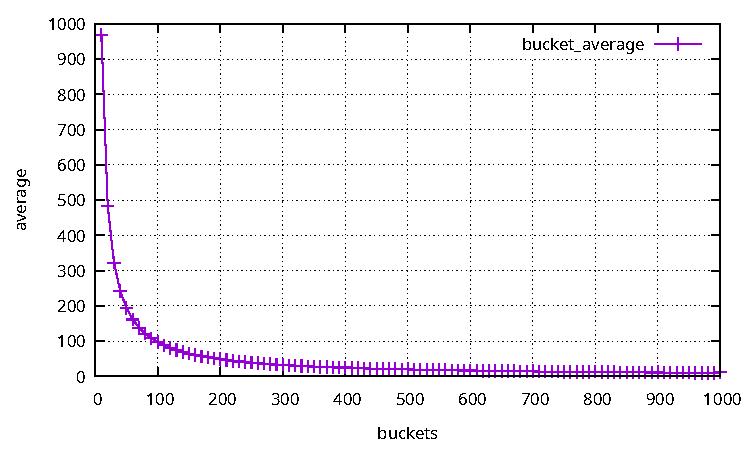
\includegraphics[scale=0.8]{graphs/bucket_average.pdf}
		\caption{
			Graph showing the average number of bucket loop throughs for a varying number of buckets.
		}
	\end{figure}
	As expected, the graph shows that the number of loop throughs per bucket decreases as the number of buckets increases.
	The number of buckets that I chose to further examine was 19412, since that was the modulos value that I found resulted in the least number of collisions (for those I tested).
	The lookup times for that number of buckets can be seen below:
	\begin{figure}[H]
		\centering
		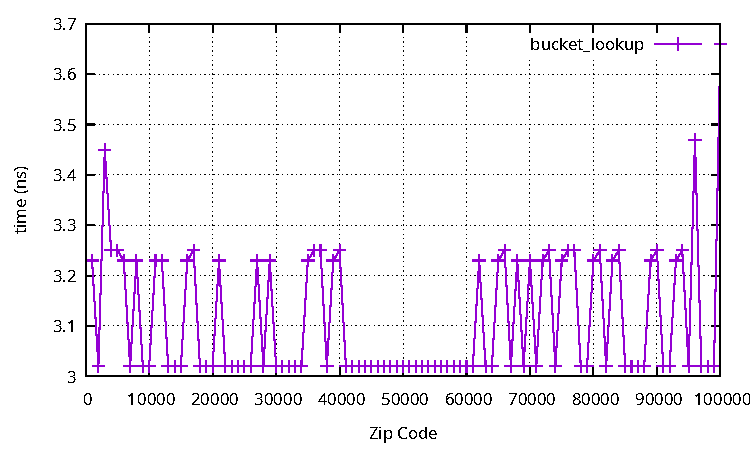
\includegraphics[scale=0.8]{graphs/bucket_lookup.pdf}
		\caption{
			Graph showing the time it took to look up different zip codes in the hash map consisting of 19412 buckets.
		}
	\end{figure}
	The jumps are most likely caused by cases where there are several elements in a single bucket, but overall the time complexity is basically \(O(1)\).

\section{Continuous Array}
	Another way to handle collisions would be to only use one array, but have it big enough so you can have elements that map to the same hash next to each other.
	This is known as \textit{linear probing}.
	The lookup procedure can then go directly to the hashed index and start traversing the array from there until it runs into the value it is looking for,
	or an unoccupied space (which means it can stop looking because the value has not been added).
	\begin{figure}[H]
		\centering
		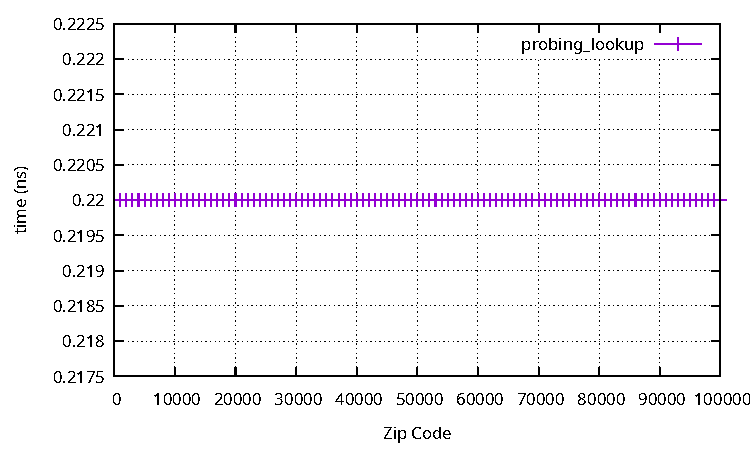
\includegraphics[scale=0.8]{graphs/probing_lookup.pdf}
		\caption{
			Graph showing the time it took to look up different zip codes in the continuous hash map using linear probing.
		}
	\end{figure}
	We see that this approach yields very promising results.
	The time it takes is now down to what we saw in the array acceses of \textbf{Table 2}.
	Here the time complexity is \(O(1)\), and the reason for it being so much faster is because we now get to access the array instantly without anything in the way (like with the buckets).

\section{Source Code}
	If anyone is interested, the source code for this project can be found over at:
	\url{https://github.com/neogulgul/ID1021/tree/main/hash}

\end{document}
